% flashcards-title: A hundred grid with some squares shaded
% flashcards-desc: A large square divided into ten rows of ten equal small squares. The top two rows are fully shaded with a pale tint and diagonal hatching, along with the first seven squares of the third row; the remaining squares are plain.
\documentclass[tikz]{standalone}
\usetikzlibrary{arrows.meta,patterns}

\definecolor{qraNavy}{HTML}{17324D}
\definecolor{qraBlue}{HTML}{2B6CB0}
\definecolor{qraGold}{HTML}{B7791F}
\definecolor{qraPale}{HTML}{EAF2F8}
\definecolor{qraGray}{HTML}{5C6773}

\tikzset{
  qra axis/.style={draw=qraNavy, line width=1.2pt},
  qra tick/.style={draw=qraNavy, line width=1pt},
  qra guide/.style={draw=qraGray, densely dashed, line width=0.8pt},
  qra counter/.style={circle, draw=qraNavy, fill=qraPale, line width=0.9pt, minimum size=7mm, inner sep=0pt},
  qra label/.style={font=\sffamily\bfseries, text=qraNavy},
  qra small label/.style={font=\sffamily, text=qraNavy},
}

\begin{document}
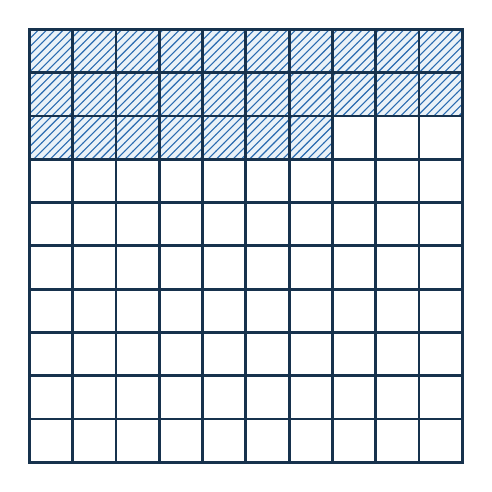
\begin{tikzpicture}[x=0.55cm, y=0.55cm]
  % Shaded region: top two rows (y from 8 to 10) plus 7 squares of the third row
  \fill[qraPale] (0,8) rectangle (10,10);
  \fill[qraPale] (0,7) rectangle (7,8);
  \path[pattern=north east lines, pattern color=qraBlue] (0,8) rectangle (10,10);
  \path[pattern=north east lines, pattern color=qraBlue] (0,7) rectangle (7,8);
  % Interior grid lines
  \foreach \i in {1,...,9} {
    \draw[qra tick] (\i,0) -- (\i,10);
    \draw[qra tick] (0,\i) -- (10,\i);
  }
  % Outer border
  \draw[qra axis] (0,0) rectangle (10,10);
\end{tikzpicture}
\end{document}
